\newpage

%%%%%%%%%%%%%%%%%%%%  解答（旧 prob_p120_2〜p126_1.png）  %%%%%%%%%%%%%%%%%%%%
\setlength{\columnseprule}{0.4pt}
\begin{multicols}{2}
\raggedcolumns

{\gtfamily\large 第15回　気体分子運動論}\par\vspace{2mm}

\Rank{A問題}
\MonN{10}{基本事項の確認}\par\nopagebreak
\begin{sisin}
ボルツマン定数の定義式をよく覚えておこう．また，気体の内部エネルギーの式$U=\dfrac{3}{2}nRT$は単原子分子理想気体に対してしか成立しないが，気体分子の二乗平均速度$\sqrt{\overline{v^2}}=\sqrt{\dfrac{3RT}{M}}$は理想気体でさえあれば成立し，二原子分子などに対しても利用できる式である．二乗平均速度の公式を利用する際には，分子量を$\U{kg/mol}$の単位にしてから$M$に代入することを忘れないようにせよ．
\end{sisin}
\KaiHead
\begin{komon}
\ko{1} ボルツマン定数は気体1分子あたりの気体定数といえるので，
       \[k_{\mathrm{B}}=\frac{R}{N_{\mathrm{A}}}=\frac{8.31}{6.02\times 10^{23}}\]
       \hspace*{2zw}$\fallingdotseq 1.38\times 10^{-23}\U{J/K}$\Ans
\ko{2} 酸素分子$\mathrm{O_2}$の分子量は$32\U{g/mol}$であるから，$M=32\times 10^{-3}\U{kg/mol}$である．よって，
       \[\sqrt{\overline{v^2}}=\sqrt{\frac{3RT}{M}}=\sqrt{\frac{3\cdot 8.31\cdot 300}{32\times 10^{-3}}}\]
       \hspace*{2zw}$\fallingdotseq 4.83\times 10^2\U{m/s}$\Ans
\ko{3} $1\U{mol}$あたりの内部エネルギーを考えると，ヘリウムは単原子分子であるから，
       \[U=\frac{3}{2}\times 1\cdot R\cdot 300\U{J}\]
       これはヘリウム気体分子の運動エネルギーの総和ゆえ，一分子あたりの平均運動エネルギーは，
       \[E=\frac{U}{N_{\mathrm{A}}}=\frac{3}{2}\cdot\frac{R}{N_{\mathrm{A}}}\cdot 300=\frac{3}{2}k_{\mathrm{B}}\cdot 300\]
       \hspace*{2zw}$\fallingdotseq 6.21\times 10^{-21}\U{J}$\Ans
\ko{4} $T\to T+10\U{K}$へ温度上昇するときの内部エネルギーの増加量は，(変化後)$-$(変化前)を求めて，
       \[\Delta U=\frac{3}{2}nR\cdot(T+10)-\frac{3}{2}nRT\]
       \hspace*{2zw}$=\dfrac{3}{2}\cdot 0.20\cdot 8.31\cdot 10\fallingdotseq 24.9\U{J}$\Ans
\end{komon}

\Rank{B問題}
\MonN{11}{気体分子運動論}\par\nopagebreak
\begin{sisin}
気体分子運動論の問題を解く際に，ミスしやすい点を以下に挙げる．これらのキーポイントをミスしないように注意すること．
\begin{komon}
\ko{1} 分子が壁$\mathrm{A}$に与えた力積と，壁$\mathrm{A}$が分子に与えた力積とを混同してはならない．分子の運動量変化から求められるのは分子が受けた力積，すなわち壁$\mathrm{A}$が分子に与えた力積である．作用・反作用の法則より，分子が壁$\mathrm{A}$に与えた力積は，壁$\mathrm{A}$が分子に与えた力積と等大逆向きである．
\ko{2} 分子が壁$\mathrm{A}$に衝突してから再び壁$\mathrm{A}$に衝突するには，分子は容器内を\underline{往復し}\hskip0pt\underline{なけれ}\hskip0pt\underline{ばなら}\hskip0pt\underline{ない}．各分子の速度成分の大きさは弾性衝突によって変化せず，速さは一定とみなしてよいので，例えば$x$軸方向に往復分$2l$の道のりを動くのに要する時間は$\dfrac{2l}{v_x}$となる．
\ko{6} 力積と力とを混同してはならない．力積とは平均の力$\times$時間であるから，力積から力を計算するには，力積を作用していた時間で割る必要がある．
\end{komon}
\end{sisin}
\KaiHead
\begin{komon}
\ko{1} 分子と壁$\mathrm{A}$との衝突は完全弾性衝突であるから，衝突前後でこの分子の速度は$x$成分のみが$v_x$から$-v_x$へ変化する．よって衝突による分子の運動量ベクトルの変化は，
       \[\begin{aligned}
         \Delta\overrightarrow{p}&=m\begin{pmatrix}-v_x\\ v_y\\ v_z\end{pmatrix}-m\begin{pmatrix}v_x\\ v_y\\ v_z\end{pmatrix}\\[1mm]
         &=\begin{pmatrix}-2mv_x\\ 0\\ 0\end{pmatrix}
       \end{aligned}\]
       であり，これは壁$\mathrm{A}$が分子に対して与えた力積である．ここで作用・反作用の関係より，衝突の際に分子が壁$\mathrm{A}$に対して与えた力積$\overrightarrow{I_m}$は，壁$\mathrm{A}$が分子に対して与えた力積と等大逆向きになるので，
       \[\overrightarrow{I_m}=-\begin{pmatrix}-2mv_x\\ 0\\ 0\end{pmatrix}=\begin{pmatrix}2mv_x\\ 0\\ 0\end{pmatrix}\]
       である．よって，大きさは$2mv_x\U{N\cdot s}$\Ans
\ko{2} 壁$\mathrm{A}$に衝突した後，分子が$x$軸方向に往復分の$2l$の道のりを進むと，再び壁$\mathrm{A}$に衝突する．分子の$x$軸方向の速さは，衝突によらず一定値$v_x$であるから，一往復に要する時間は$\dfrac{2l}{v_x}$である．よって，この分子は$t\U{s}$間に壁$\mathrm{A}$と$\dfrac{v_xt}{2l}$回衝突する．\par
       \hspace*{1zw}以上と(1)より，$t\U{s}$間にこの分子が壁$\mathrm{A}$に対して及ぼす力積の大きさは，
       \[2mv_x\cdot\frac{v_xt}{2l}=\frac{mv_x^2t}{l}\U{N\cdot s}\Ans\]
\ko{3} 各分子ごとに速度の$x$成分の二乗値の$v_x^2$が異なるので，(2)で求めた，$t\U{s}$間に分子が壁$\mathrm{A}$に対して及ぼす力積の大きさは分子ごとに異なるが，$v_x^2$の平均値を$\overline{v_x^2}$とすると，$t\U{s}$間に壁$\mathrm{A}$に対して及ぼす力積の大きさの平均値は，一分子あたり
       \[\frac{m\overline{v_x^2}t}{l}\U{N\cdot s}\]
       である．全分子は$N$個だから，
       \[I=N\frac{m\overline{v_x^2}t}{l}\U{N\cdot s}\Ans\]
\ko{4} $v$と$v_x$, $v_y$, $v_z$の間には三平方の定理より
       \[v^2=v_x^2+v_y^2+v_z^2\]
       が成立する．全分子に対して両辺それぞれ平均を取ると，
       \[\overline{v^2}=\overline{v_x^2}+\overline{v_y^2}+\overline{v_z^2}\]
       が成立する．また気体分子運動の等方向性より，各軸方向の速度成分の二乗の平均値の間に，
       \[\overline{v_x^2}=\overline{v_y^2}=\overline{v_z^2}\]
       が成立する．以上より，
       \[\overline{v_x^2}=\frac{1}{3}\overline{v^2}\Ans\]
\ko{5} (3)(4)を用いて，
       \[I=\frac{Nm\cdot\frac{1}{3}\overline{v^2}\cdot t}{l}=\frac{Nm\overline{v^2}t}{3l}\U{N\cdot s}\Ans\]
\ko{6} 壁$\mathrm{A}$が全分子から受ける平均の力を$\overline{F}\U{N}$とすれば，平均の力の定義より，$I$, $\overline{F}$, $t$の間に
       \[I=\overline{F}\cdot t\]
       が成り立つ．よって，
       \[\overline{F}=\frac{I}{t}=\frac{Nm\overline{v^2}}{3l}\U{N}\Ans\]
\ko{7} 壁$\mathrm{A}$の面積は$l^2$であるから，気体の圧力は
       \[p=\frac{\overline{F}}{l^2}=\frac{Nm\overline{v^2}}{3l^3}\U{Pa}\Ans\]
\ko{8} (7)および$V=l^3$より，
       \[p=\frac{Nm\overline{v^2}}{3V}\]
       これより，
       \[pV=\frac{Nm\overline{v^2}}{3}\Ans\]
\end{komon}

\MonN{12}{気体分子運動論}\par\nopagebreak
\begin{sisin}
前問で得られたベルヌーイの式は，気体分子運動と気体の圧力を結びつける式である．一方，理想気体の状態方程式$pV=nRT$は気体の圧力と気体の温度とを結びつける式である．よって，この二つを組み合わせれば，気体の温度と気体の分子運動（二乗平均速度など）とを結びつけることができる．あとはこれによって得られた式を，問題条件で要求されている変数にうまく置き換えていこう．
\end{sisin}
\KaiHead
\begin{komon}
\ko{1} 気体分子運動論のベルヌーイの式より，
       \[pV=\frac{Nm\overline{v^2}}{3}\]
       である．またこの理想気体の物質量は$n=\dfrac{N}{N_{\mathrm{A}}}\U{mol}$であるから，状態方程式は，
       \[pV=\frac{N}{N_{\mathrm{A}}}RT\]
       である．以上2式の両辺を結ぶと
       \[\frac{Nm\overline{v^2}}{3}=\frac{N}{N_{\mathrm{A}}}RT\]
       であり，これを変形すると，
       \[\overline{v^2}=\frac{3RT}{mN_{\mathrm{A}}}\]
       となる．ここで，$mN_{\mathrm{A}}$は気体分子$1\U{mol}$あたりの質量$M\U{kg/mol}$を表しているので，
       \[\overline{v^2}=\frac{3RT}{M}\]
       である．以上より，
       \[\sqrt{\overline{v^2}}=\sqrt{\frac{3RT}{M}}\U{m/s}\Ans\]
\ko{2} 密度$\rho$は，単位体積当たりの質量である．気体分子の全質量は$M\cdot n\U{kg}$であるから，
       \[\rho=\frac{M\cdot n}{V}\U{kg/m^3}\]
       であるが，状態方程式$pV=nRT$より$\dfrac{p}{RT}=\dfrac{n}{V}$であるから，
       \[\rho=\frac{pM}{RT}\U{kg/m^3}\]
       と表せる．よって，$\dfrac{RT}{M}=\dfrac{p}{\rho}$であるから，(1)で得られた答を書き換えて，
       % 誤植訂正（2026-08-31）：原本は「(2)で得られた答を書き換えて」だが，
       %   書き換えているのは(1)の答なので「(1)」に改めた．
       \[\sqrt{\overline{v^2}}=\sqrt{\frac{3p}{\rho}}\U{m/s}\Ans\]
\ko{3} 気体分子の平均運動エネルギー$\overline{E}$は，
       \[\begin{aligned}
         \overline{E}&=\frac{1}{2}m\overline{v^2}=\frac{1}{2}m\cdot\frac{3RT}{M}=\frac{1}{2}m\cdot\frac{3RT}{mN_{\mathrm{A}}}\\[1mm]
         &=\frac{3RT}{2N_{\mathrm{A}}}
       \end{aligned}\]
       と表せる．
       \[k_{\mathrm{B}}=\frac{R}{N_{\mathrm{A}}}\]
       を用いて$\overline{E}$を書き換えると，
       \[\overline{E}=\frac{3}{2}k_{\mathrm{B}}T\U{J}\Ans\]
\end{komon}
\begin{chuu}
A問題においては，ヘリウム一分子が持つ運動エネルギーを，気体の内部エネルギー$U=\dfrac{3}{2}nRT$を気体の分子数で割り算することによって求めたが，\underline{この方}\hskip0pt\underline{法は単}\hskip0pt\underline{原子分}\hskip0pt\underline{子理想}\hskip0pt\underline{気体で}\hskip0pt\underline{なけれ}\hskip0pt\underline{ば利用}\hskip0pt\underline{するこ}\hskip0pt\underline{とがで}\hskip0pt\underline{きない}．なぜなら，気体の内部エネルギーの結果式$U=\dfrac{3}{2}nRT$は単原子分子理想気体でなければ成立しないからである．ところが，本問で導いた気体分子一分子あたりの平均運動エネルギー
\[\overline{E}=\frac{3}{2}k_{\mathrm{B}}T\U{J}\]
\underline{の式は}\hskip0pt\underline{単原子}\hskip0pt\underline{分子理}\hskip0pt\underline{想気体}\hskip0pt\underline{でなく}\hskip0pt\underline{ても成}\hskip0pt\underline{立する}．なぜなら，この式を導くのに利用した式はすべて理想気体でさえあれば成立する式だからである．すなわち，単原子分子理想気体でない場合について，気体分子1分子あたりの平均運動エネルギーを求めよと問われた場合には，内部エネルギーの割り算という考え方から求めるのは間違いであり，必ず\underline{気体分}\hskip0pt\underline{子運動}\hskip0pt\underline{論によ}\hskip0pt\underline{るベル}\hskip0pt\underline{ヌーイ}\hskip0pt\underline{の式を}\hskip0pt\underline{元にし}\hskip0pt\underline{て考え}\hskip0pt\underline{なけれ}\hskip0pt\underline{ばなら}\hskip0pt\underline{ない}．
\end{chuu}
\begin{itembox}[l]{【参考】}
では2原子分子の場合，内部エネルギーの式を気体の総分子数で割り算して出てくる答えはどうなるのかを考えてみよう．2原子分子の場合，内部エネルギーの式は
\[U=\frac{5}{2}nRT\U{J}\]
である．これを気体分子数$N=n\cdot N_{\mathrm{A}}$で割り算して気体分子一分子あたりが持つエネルギーを求めると，
\[\frac{U}{N}=\frac{5}{2}k_{\mathrm{B}}T\U{J}\]
となる．(3)で求めたように，気体分子の運動エネルギーは
\[\overline{E}=\frac{3}{2}k_{\mathrm{B}}T\U{J}\]
であるから，気体分子一分子あたりが持つエネルギーはこれよりも$k_{\mathrm{B}}T\U{J}$だけ多い．このエネルギーの正体は，実は気体分子がその内部で回転運動することによって持つエネルギーである．単原子分子の場合には内部回転というものは存在しないため，気体分子の運動エネルギー$\overline{E}=\dfrac{3}{2}k_{\mathrm{B}}T\U{J}$がそのまま気体分子一分子あたりが持つエネルギーとなるが，2原子分子以上になると，気体分子内回転が存在するため，回転によって持つエネルギーを加えたものが気体分子一分子あたりが持つエネルギーとなる．
\end{itembox}

\MonN{13}{気体分子運動論の利用}\par\nopagebreak
\begin{sisin}
前問・前々問で導出した気体分子運動の二乗平均速度の式$\sqrt{\overline{v^2}}=\sqrt{\dfrac{3RT}{M}}\U{m/s}$を利用して考えていけばよい．$M$に分子量を代入する際には，単位を$\U{kg/mol}$に換算してから代入することに注意せよ．
\end{sisin}
\KaiHead
\begin{komon}
\ko{1} 気体分子運動の二乗平均速度の式
       \[\sqrt{\overline{v^2}}=\sqrt{\frac{3RT}{M}}\U{m/s}\]
       に各値を代入して求めると，
       \[\sqrt{\overline{v^2}}=\sqrt{\frac{3\cdot 8.3\cdot 300}{28\times 10^{-3}}}\]
       \hspace*{2zw}$\fallingdotseq 5.2\times 10^2\U{m/s}$\Ans
\ko{2} 二乗平均速度の式より，温度$T$が共通であれば，気体分子運動の速さは$\dfrac{1}{\sqrt{M}}$に比例する．また，ヘリウム・ネオンは希ガスで単原子分子であるから，分子量＝原子量である．よって，二つの気体の二乗平均速度の比は，
       \[\begin{aligned}
         \sqrt{\overline{v_{\mathrm{He}}^2}}:\sqrt{\overline{v_{\mathrm{Ne}}^2}}
         &=\frac{1}{\sqrt{M_{\mathrm{He}}}}:\frac{1}{\sqrt{M_{\mathrm{Ne}}}}\\[1mm]
         &=\frac{1}{\sqrt{4}}:\frac{1}{\sqrt{20}}
       \end{aligned}\]
       である．以上より，平均運動エネルギー$\overline{E}=\dfrac{1}{2}m\overline{v^2}$の比は，
       \[\begin{aligned}
         \overline{E_{\mathrm{He}}}:\overline{E_{\mathrm{Ne}}}
         &=\frac{1}{2}m_{\mathrm{He}}\overline{v_{\mathrm{He}}^2}:\frac{1}{2}m_{\mathrm{Ne}}\overline{v_{\mathrm{Ne}}^2}\\[1mm]
         &=m_{\mathrm{He}}N_{\mathrm{A}}\overline{v_{\mathrm{He}}^2}:m_{\mathrm{Ne}}N_{\mathrm{A}}\overline{v_{\mathrm{Ne}}^2}\\[1mm]
         &=4\cdot\frac{1}{4}:20\cdot\frac{1}{20}\\[1mm]
         &=1:1
       \end{aligned}\]
       である．よって，1分子あたりの平均運動エネルギーは同じである．\Ans
\end{komon}
\begin{bekkai}
前問の，1分子あたりの平均運動エネルギーの式
\[\overline{E}=\frac{3}{2}k_{\mathrm{B}}T\U{J}\]
を覚えていれば答えは明らかである．この式は分子量を含まず，$T$のみを変数として含むので，1分子あたりの平均運動エネルギーは温度のみによって決まる．よって，温度が同じであれば1分子あたりの平均運動エネルギーは同じである．\par
\hspace*{1zw}この式を覚えていない場合，問題文で問われているのが単原子分子気体であることに着目して考えることも可能である．単原子分子気体であれば，前問の注意で述べたように1分子あたりの平均運動エネルギーを，内部エネルギーの式/気体分子数によって求めることができるので，
\[\overline{E}=\frac{U}{N}=\frac{\frac{3}{2}nRT}{n\cdot N_{\mathrm{A}}}=\frac{3}{2}\cdot\frac{R}{N_{\mathrm{A}}}T\U{J}\]
と求められる．後は上述と同じ議論をすればよい．
\end{bekkai}
\begin{komon}
\ko{3} $\sqrt{\overline{v^2}}=\sqrt{\dfrac{3RT}{M}}\U{m/s}$の式より，気体分子の二乗平均速度は$\sqrt{T}$に比例している．よって，温度$T\U{K}$が$273\U{K}$から$273+273=546\U{K}$へと変化した際には，二乗平均速度は$\sqrt{2}$倍になる．\Ans\par
       \hspace*{1zw}また，1分子あたりの平均運動エネルギーは，
       \[\overline{E}=\frac{1}{2}m\overline{v^2}\]
       で与えられるのだから，二乗平均速度の二乗に比例して変化する．よって，二乗平均速度が$\sqrt{2}$倍になれば平均運動エネルギーは2倍になる．\Ans
\end{komon}
\begin{bekkai}
もちろん後者については$\overline{E}=\dfrac{3}{2}k_{\mathrm{B}}T\U{J}$の式を利用して2倍と答えてもよい．
\end{bekkai}
\begin{breakbox}\noindent{\gtfamily 【参考】}\par\nopagebreak
本問の(1)〜(3)では，理想気体の気体分子の二乗平均速度$\sqrt{\overline{v^2}}=\sqrt{\dfrac{3RT}{M}}\U{m/s}$の式をフル活用して答えを導いているが，この式は利用する機会が少ないこともあり，意外と忘れがちである．以下のように考えると簡単に導くことができるので，覚えておくとよい．\par
\hspace*{1zw}まず，$n\U{mol}$の単原子分子理想気体を考える．単原子分子理想気体であれば，その内部エネルギーは
\[U=\frac{3}{2}nRT\U{J}\]
で与えられる．単原子分子理想気体ではその内部エネルギーとは原子の持つ運動エネルギーの総和のことだから，1分子あたりの平均運動エネルギー$\dfrac{1}{2}m\overline{v^2}$と全分子数$nN_{\mathrm{A}}$との積が内部エネルギー$U$となる．よって，
\[U=(nN_{\mathrm{A}})\times\frac{1}{2}m\overline{v^2}\]
\hspace*{1zw}これらを結んで解くと，
\[\sqrt{\overline{v^2}}=\sqrt{\frac{3RT}{mN_{\mathrm{A}}}}\]
が導かれる．ただし$m$は原子一つあたりの質量（{\gtfamily kg}単位）である．式の中に出てくる$mN_{\mathrm{A}}$は$1\U{mol}$あたりの分子の質量を表していることになるので，$1\U{mol}$あたりの分子の質量を$M\U{kg/mol}$で表すと$M=mN_{\mathrm{A}}$であるから
\[\sqrt{\overline{v^2}}=\sqrt{\frac{3RT}{M}}\]
として二乗平均速度の式を導くことが可能となる．\par
\hspace*{1zw}以上の議論では単原子理想気体であることを用いているが，結論の式である
\[\sqrt{\overline{v^2}}=\sqrt{\frac{3RT}{M}}\]
は，\underline{単原子}\hskip0pt\underline{分子理}\hskip0pt\underline{想気体}\hskip0pt\underline{でなく}\hskip0pt\underline{とも成}\hskip0pt\underline{立する}．二乗平均速度は気体分子運動論から導出されるものであり，単原子分子気体を仮定せずとも導出できるからである．\par
\hspace*{1zw}また，
\[\frac{1}{2}m\overline{v^2}\times(nN_{\mathrm{A}})=\frac{3}{2}nRT=\frac{3}{2}PV\]
と変形すれば簡単にベルヌーイの式を導出することができる．検算の方法として覚えておくとよい．
\end{breakbox}

\MonN{14}{内部エネルギー}\par\nopagebreak
\begin{sisin}
この気体は単原子分子理想気体であるから，内部エネルギーは$U=\dfrac{3}{2}nRT$と表せる．この式から分かるように，\underline{理想気}\hskip0pt\underline{体の内}\hskip0pt\underline{部エネ}\hskip0pt\underline{ルギー}\hskip0pt\underline{は温度}\hskip0pt\underline{のみに}\hskip0pt\underline{依存す}\hskip0pt\underline{る}ので，温度・圧力・体積などの変化によって内部エネルギーがどう変化するのかを考える際には，温度がどう変化するかさえ考えればよい．
\end{sisin}
\KaiHead
\begin{komon}
\ko{1} 気体の内部エネルギー$U$は$U=\dfrac{3}{2}nRT\U{J}$と表される．\par
       \hspace*{1zw}ここで，温度を一定に保てば（$U=\dfrac{3}{2}nRT\U{J}$の式は変化しないので）体積を変化させても内部エネルギーは変わらず，1倍のままである．\Ans
\ko{2} 状態方程式$PV=nRT$の式より，圧力を一定に保って体積を$m$倍にするときは温度が$m$倍になる．\par
       \hspace*{1zw}よって，温度が$m$倍になれば，内部エネルギーも$m$倍になる．\Ans
\end{komon}
\begin{bekkai}
シャルルの法則より，体積と温度は比例する．内部エネルギーは温度に比例するので，体積が$m$倍になるとき，内部エネルギーも$m$倍になる．\Ans
\end{bekkai}
\begin{komon}
\ko{3} 箱に封入された気体のモル数を$n'\U{mol}$とする．初めの状態における，この気体の状態方程式は
       \[PV=n'RT\]
       であるから，この箱に封入された気体のモル数は
       \[n'=\frac{PV}{RT}\U{mol}\]
       で与えられる．この気体の温度は$\Delta T=T'-T$だけ上昇したので，この変化による内部エネルギーの増加$\Delta U$は
       \[\Delta U=\frac{3}{2}n'RT'-\frac{3}{2}n'RT=\frac{3}{2}n'R\cdot\Delta T\]
       で与えられる（変化後$-$変化前で増加量が求められる）．ここで，熱力学第一法則を考えると，気体は仕事のやり取りをしていないから，気体に対して与えた熱量$Q\U{J}$はすべて内部エネルギーの増加$\Delta U$に利用されたと考えられる．よって，熱力学第一法則を表す式は，
       \[Q=\Delta U\]
       である．これを解いて，
       \[\Delta T=\frac{2Q}{3n'R}=\frac{2Q}{3PV}T\U{K}\Ans\]
\ko{4} 状態変化後の気体の状態方程式を立てると，
       \[P'V=n'RT'\]
       である．これと(3)の答より，
       \[\begin{aligned}
         P'&=\frac{n'RT'}{V}=\frac{n'R(T+\Delta T)}{V}=\frac{P}{T}(T+\Delta T)\\[1mm]
         &=P+P\frac{\Delta T}{T}=P+\frac{2Q}{3V}\U{Pa}\Ans
       \end{aligned}\]
\end{komon}

\MonN{15}{$p-V$図}\par\nopagebreak
\begin{sisin}
まず初めに各点での状態方程式を立てて，その圧力，体積を求めてしまい，それからそれらの点を結んでいくとよい．\par
\hspace*{1zw}ただし，$T-V$図上での変化が直線的だからといって，$p-V$図上の変化も直線的であるとは限らない．どのような曲線の上に乗って変化していくかについては，状態方程式$pV=nRT$の式からその変化中に一定であるものをはじき出して考えるとよい．$\mathrm{B}\to\mathrm{C}$では一定の変数がないので，状態方程式と，$T$と$V$の関係式を整理して考えよ．
\end{sisin}
\KaiHead
\hspace{1zw}気体の物質量を$n\U{mol}$とし，$\mathrm{B}$, $\mathrm{C}$における気体の圧力をそれぞれ$p_{\mathrm{B}}\U{Pa}$, $p_{\mathrm{C}}\U{Pa}$とする．\par
\hspace{1zw}$\mathrm{A}$，$\mathrm{B}$，$\mathrm{C}$各点での気体の状態方程式は，
\[\mathrm{A}:2p_0\cdot V_0=nR\cdot 2T_0\]
\[\mathrm{B}:p_{\mathrm{B}}\cdot 2V_0=nR\cdot 2T_0\]
\[\mathrm{C}:p_{\mathrm{C}}\cdot V_0=nR\cdot T_0\]
となる．これらの式を解くと，
\[n=\frac{p_0V_0}{RT_0},\ p_{\mathrm{B}}=p_0,\ p_{\mathrm{C}}=p_0\]
が得られる．よって，$\mathrm{A}$，$\mathrm{B}$，$\mathrm{C}$は$p-V$図上では次図のような位置にくる点である．
\begin{center}
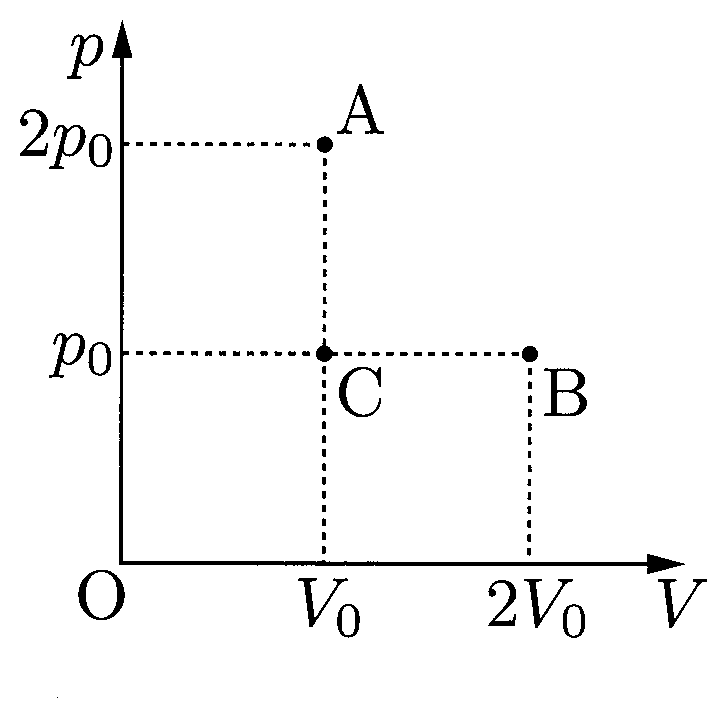
\includegraphics[keepaspectratio,width=34mm]{fig/ch15_p124_pv.png}
\end{center}
\hspace{1zw}各状態変化をそれぞれ考える．
\begin{komon}
\ko{1} $\mathrm{A}\to\mathrm{B}$の状態変化\par
       \hspace*{1zw}この変化において気体の温度は一定であるから，理想気体の状態方程式より，$pV=nRT=$一定となる．よって，体積が$V\U{m^3}$になったときの気体の圧力を$p(V)\U{Pa}$とすれば，$\mathrm{A}$点との間に
       \[p(V)\cdot V=2p_0\cdot V_0\]
       の関係が成立する．よって，
       \[p(V)=2p_0V_0\frac{1}{V}\U{Pa}\quad\left(\propto\frac{1}{V}\right)\]
       となり，$p-V$図上では双曲線を描いて変化する．
\ko{2} $\mathrm{B}\to\mathrm{C}$の変化\par
       \hspace*{1zw}この変化途中の，温度，体積がそれぞれ$(T,\ V)$の状態のときの気体の圧力を$p(V)\U{Pa}$とおく．グラフより，体積と温度は
       \[T=\frac{T_0}{V_0}V\]
       の関係を保ちつつ，$T=2T_0\to T_0\U{K}$（$V=2V_0\to V_0\U{m^3}$）まで変化する．また，$(p(V),\ T,\ V)$のときの状態方程式より，
       \[p(V)\cdot V=nRT\]
       が成立するので，以上2式を整理すると，
       \[p(V)=nR\frac{T_0}{V_0}=p_0\]
       となり，変化途中の気体の体積$V$によらず，圧力は常に$p_0\U{Pa}$となる．すなわち，この変化は定圧変化であり，$\mathrm{B}\to\mathrm{C}$へは$p=p_0$の直線上を$V=2V_0\to V_0\U{m^3}$まで変化する．
\ko{3} $\mathrm{C}\to\mathrm{A}$の状態変化\par
       \hspace*{1zw}この変化では，与えられた$T-V$グラフより体積が一定値のまま変化するので，$\mathrm{C}\to\mathrm{A}$へは$V=V_0$の直線上を変化していく．
\end{komon}
\hspace{1zw}以上をまとめると，この状態変化の$p-V$図は次図のようになる．
\begin{center}
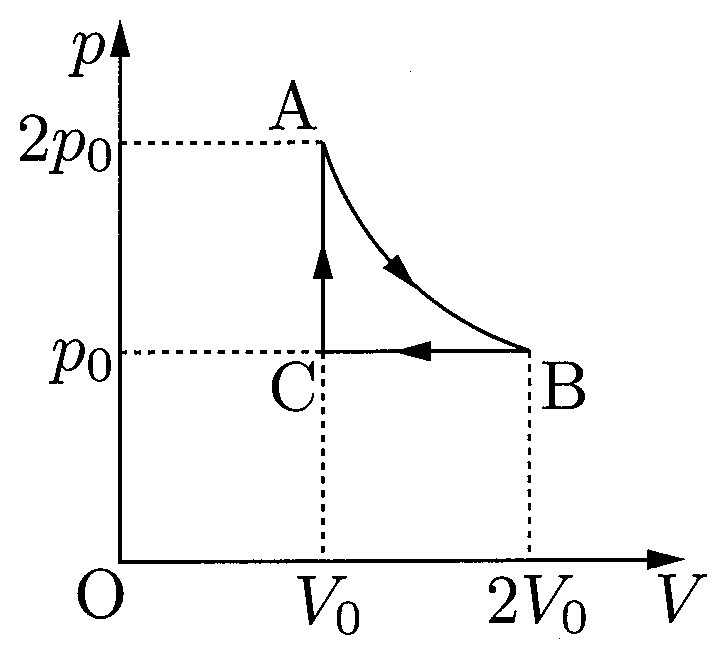
\includegraphics[keepaspectratio,width=34mm]{fig/ch15_p125_pv.png}
\end{center}
\hspace*{\fill}\Ans

\Rank{C問題}
\MonN{16}{球内での気体分子運動論}\par\nopagebreak
\begin{sisin}
考え方の指針は直方体容器の場合と全く変わらない．\MARU{1}1回あたりの衝突で壁面に与える力積を求める，\MARU{2}時間$t\U{s}$間での衝突回数および与える力積を求める，\MARU{3}力積と力の関係，および全分子について与える力積を考えて，壁面に作用する力を求める，\MARU{4}気体分子運動の等方向性を利用，\MARU{5}圧力を計算する，という流れである．（本問の場合はすべての分子が同じ速さと考えて分子ごとのバラつきを考えていないため，\MARU{4}は不要）
\end{sisin}
\KaiHead
% 誤植訂正（2026-08-31）：原本の解答は (1)(2) の次が (1)(2)(3)…(7) と振り直されており，
%   問題文の空欄番号（1〜9）と2つずれていた．空欄番号に合わせて (3)〜(9) に改めた．
\begin{komon}
\item[{\makebox[1.9zw][r]{(1)(2)}}] 分子と壁との衝突は完全弾性衝突であるから，衝突前後で点$\mathrm{B}$における接線方向，すなわち半径$\mathrm{OB}$に垂直な方向の速度成分は変化せず，$\mathrm{OB}$方向の速度成分が反転して$v\cos\theta$から$-v\cos\theta$へ変化する．よって，衝突によるこの分子の運動量の変化は，$\mathrm{O}$から$\mathrm{B}$の方向を正として，
       \[m\cdot(-v\cos\theta)-m\cdot v\cos\theta=-2mv\cos\theta\]
       となる．よって，(1)$\ \overrightarrow{\mathrm{BO}}$ベクトルの方向に，大きさ(2)$\ 2mv\cos\theta\U{N\cdot s}$\Ans
\ko{3} 次の衝突点は$\mathrm{C}$であるが，$\mathrm{B}$点での衝突は弾性衝突であるから，$\angle\mathrm{ABO}=\angle\mathrm{OBC}=\theta$である．よって，$\mathrm{B}\to\mathrm{C}$までの距離は，図より
       \[\overline{\mathrm{BC}}=2a\cos\theta\U{m}\]
       である．また，分子の速さは衝突前後で変化しないので，次に衝突するまでにかかる時間は
       \[\frac{\overline{\mathrm{BC}}}{v}=\frac{2a\cos\theta}{v}\U{s}\Ans\]
\ko{4} 図より明らかに$\angle\mathrm{BOC}=\theta$であるから，分子の器壁への入射角は一定である．また，分子の速さも器壁と何回衝突しても一定のままであるから，衝突時間間隔はずっと$\dfrac{2a\cos\theta}{v}\U{s}$の一定のままである．よって，時間$t\U{s}$間の間の壁面との衝突回数は
       \[t\Big/\frac{2a\cos\theta}{v}=\frac{vt}{2a\cos\theta}\,[\text{回}]\Ans\]
\ko{5} 一回の衝突によってこの気体分子が壁面に対して与える力積の大きさは，(1)・(2)の正負逆なので
       \[\text{壁面を押す方向に，大きさ}\ 2mv\cos\theta\U{N\cdot s}\]
       である．よって，時間$t\U{s}$間の間に壁面に対して与えた力積の大きさの総和は
       \[2mv\cos\theta\cdot\frac{vt}{2a\cos\theta}=\frac{mv^2}{a}t\U{N\cdot s}\Ans\]
\ko{6} 1分子あたりが(5)であるから，
       \[N\cdot\frac{mv^2}{a}t\U{N\cdot s}\Ans\]
\ko{7} 器壁に及ぼす平均の力の大きさを$\overline{F}\U{N}$とすれば，平均の力と力積との関係より，
       \[\overline{F}\cdot t=N\cdot\frac{mv^2}{a}t\]
       である．よって，器壁に対して及ぼす平均の力の大きさは
       \[\overline{F}=\frac{Nmv^2}{a}\U{N}\Ans\]
\ko{8} 容器内面の面積は$S=4\pi a^2\U{m^2}$であるから，
       \[p=\frac{\overline{F}}{S}=\frac{\dfrac{Nmv^2}{a}}{4\pi a^2}=\frac{Nmv^2}{4\pi a^3}\U{Pa}\Ans\]
\ko{9} また$V=\dfrac{4}{3}\pi a^3\U{m^3}$より，
       \[p=\frac{Nmv^2}{3V}\]
       よって，
       \[pV=\frac{Nmv^2}{3}\Ans\]
\end{komon}
\begin{itembox}[l]{【参考】}
結局，球形の容器であっても気体分子の速さの二乗と圧力との関係式は，立方体容器の場合と全く同一になる．また，これと状態方程式を組み合わせれば気体の二乗平均速度の式が立方体容器の場合と全く同様に導かれる．
\end{itembox}
\begin{itembox}[l]{【参考】}
（ここに書かれていることはかなり難しいため，興味のある人のみ読めばよい）\par
\hspace*{1zw}本問では気体分子運動の等方向性
\[\overline{v_x^2}=\overline{v_y^2}=\overline{v_z^2}\]
を利用しなかったが，この式は容器の形状によらずに成立する．\par
\hspace*{1zw}これは気体分子同士が非常に頻繁に相互に衝突しているためである．例えば$0\Cel$，1気圧下において，気体分子が他の気体分子に衝突せずに進める距離（平均自由行程という）はおよそ$10^{-7}\U{m}$程度でしかなく，およそ$10^{-19}\U{s}$程度の間隔で気体分子は衝突を繰り返している．
このため，例えば容器の一部の器壁などの移動によってある軸方向の速度成分が大きくなったとしても，気体分子相互の衝突のためすぐに他の軸方向の速度成分も増加してしまう（断熱変化を気体分子運動論に基づいて考える場合などに用いられる）．\par
\hspace*{1zw}ベルヌーイの式の導出などに用いた「気体分子相互の衝突はない」という仮定とつじつまが合わなくなってしまうように感じるかもしれないが，これについては考慮しなくてよい．というのは，本来ベルヌーイの式は統計熱力学を元にして導出されるものであり，これを高校範囲の知識だけで扱おうとするのは無理である．正しくはどうなのか，という点については大学に入ってから学べばよいが，高校範囲では次のように考えて問題を解けばよい．
\begin{komon}
\item[{\makebox[1.9zw][r]{\MARU{1}}}] ベルヌーイの式を導く際には，気体分子相互間の衝突については考慮しなくてよい．
\item[{\makebox[1.9zw][r]{\MARU{2}}}] ただし，気体分子運動の等方向性を用いる際には，気体分子の相互衝突が起こっていると考える．
\end{komon}
\end{itembox}

\end{multicols}
